\chapter{Design Decisions and Implementation}

Over the course of the development of my project, I had to make numerous design decisions for each part. 
This chapter lays out and explains the design decisions I made, along with justifications for them, and details the implementation process that followed these decisions.

\section{Version Control System}

Throughout the development of the project, I will use the industry-standard Git version control system. 
This allows me to keep snapshots of the project over time, so I can revert if anything goes wrong, as well as keeping the project backed up to GitHub.

\section{Choosing Technologies}

\subsection{Choosing a Game Engine}

To develop the game frontend, I needed to choose a game engine or game development framework. Throughout my research, I considered three different options, Godot, Unity and Pygame.
I selected Godot over Unity and Pygame after careful consideration of my project's requirements. 
While Unity offers powerful features, its proprietary nature, heavyweight installation, and steep learning curve made it less suitable for my academic project. 
Unity's reliance on the C Sharp programming language would also have required additional time investment to master. 
Pygame, despite its Python compatibility that would have allowed native interfacing with PyTorch, lacks a graphical development environment and many built-in features that would speed up development. 
In contrast, Godot offered the perfect balance: it's open-source and free, extremely lightweight (only 130MB), uses a Python-like language (GDScript) that was quick to learn, features an intuitive interface I was already familiar with, and provides excellent 2D capabilities that matched my game requirements.
Additionally, Godot's plain text resources integrate seamlessly with Git, its cross-platform compatibility ensures the game works on both Windows and Linux environments (critical for working between home and university), and its networking features provide essential connectivity to the backend model.

\subsection{Choosing an ML Framework}

For the model backend, there were only two real options - PyTorch and Tensorflow.
I chose PyTorch over TensorFlow for my machine learning framework due to several key advantages. 
While TensorFlow offers a robust ecosystem and production-ready deployment tools, PyTorch's more intuitive API and dynamic computation graph better suited the experimental nature of this project. 
TensorFlow's static graph design, though efficient for production, would have hindered the rapid prototyping and debugging I needed during development. 
PyTorch's Python-first approach also aligned better with my existing workflow, offering seamless integration with Python data science libraries like NumPy and Pandas. 
The framework's extensive documentation, community support, and built-in tools for neural network development made implementation more straightforward. 
Additionally, PyTorch's native support for GPU acceleration provided the necessary computational power for model training, and its reinforcement learning libraries offered ready-made solutions for developing game AI agents. 
TensorFlow's steep learning curve and more verbose syntax would have increased development time without providing significant benefits for this particular academic project.

\section{Design of the Game}

For the game component of my project, I decided to develop a 2D tile-based platformer, similar to Super Mario Bros. 
This decision was driven by several practical considerations. 
First, 2D platformers offer a good balance between implementation complexity and gameplay depth, making them ideal for academic projects with limited timeframes.
The tile-based approach simplifies level design, collision detection, and environmental interactions while still allowing for creative gameplay mechanics. 
The tile-based approach is also ideal for RL, as the environment is formed of tiles that can be classified by type, numbered, and then fed directly into a model.

\begin{figure}[h]
    \centering
    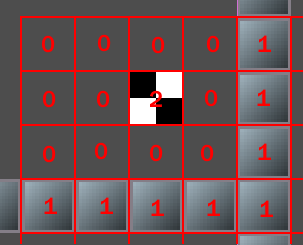
\includegraphics[width=0.8\textwidth]{figures/tilemap.png}
    \caption{Classifying tiles by type}
    \label{fig:tilemap}
\end{figure}

From a technical perspective, 2D platformers require fewer computational resources than 3D games, enabling me to focus more processing power on the machine learning components rather than graphics rendering. 
Godot's excellent 2D capabilities made this genre particularly suitable, as the engine provides robust tools for sprite animation, tilemap management, and physics-based movement.
Additionally, platformers offer clear, discrete states and actions that translate well to reinforcement learning problems. 
The character can move left, right, jump, or perform other specific actions, while the game state can be represented efficiently for the ML model to process.
This clarity in the action space makes platformers an excellent testbed for AI development, as the model must learn fundamental gaming concepts like obstacle avoidance, timing, and spatial navigation.
The tile-based structure also facilitates procedural level generation, allowing me to create varied environments for training the AI without manually designing each level. 
This was particularly important for developing robust models that could generalize across different scenarios rather than overfitting to specific level layouts.

I decided to design the game around a clear, measurable objective: completing a time-based obstacle course. This design choice was deliberate as it provides several advantages for both gameplay and AI development.
From a gameplay perspective, a timed obstacle course offers an intuitive goal that requires no elaborate explanation - players simply need to reach the end as quickly as possible. 
This straightforward objective creates natural replay value as players (human or AI) attempt to optimize their route and execution to achieve faster completion times.
From a machine learning standpoint, this objective is ideal because it creates a well-defined reward function where success can be quantified precisely through time measurements. 
The faster an agent completes the course, the better its performance, providing a clear optimization target for reinforcement learning algorithms.
This design also allows for incremental learning progression. An AI agent can first learn the fundamental task of reaching the goal, then gradually optimize for speed - mirroring how human players typically approach such challenges. 
The continuous nature of the time metric (as opposed to binary success/failure) gives the learning algorithm more nuanced feedback about small improvements in performance.
Additionally, timed courses naturally incorporate key platforming challenges like precise jumping, obstacle avoidance, and route optimization, creating a rich environment for AI learning while remaining accessible to human players for comparison.

\section{Building a Basic Game Environment}

My first task was to build a basic game environment within Godot that could then be built further upon.
This consists of:
\begin{itemize}
    \item \textbf{Player Character}: I implemented a character with basic movement controls including running left/right, jumping, and falling with appropriate physics, using Godot's built in 2D physics system.
    \item \textbf{Camera}: The game's camera is a Camera2D node that remains static providing a view of the whole map.
    \item \textbf{Tile Based Map}: I created a tilemap system using Godot's TileMapLayer node, allowing me to construct levels from reusable tiles representing walls, floors and ceilings.
    \item \textbf{Kill Plane}: At the bottom of the map, there is a player collidable box that will reset their position if it is touched. This ensures that the player cannot fall out of the map endlessly.
    \item \textbf{Finish Line and Timer}: Each map contains a finish line tile. As soon as the player is instantiated, their timer starts and will stop once they touch the finish line.
\end{itemize}

\begin{figure}[h]
    \centering
    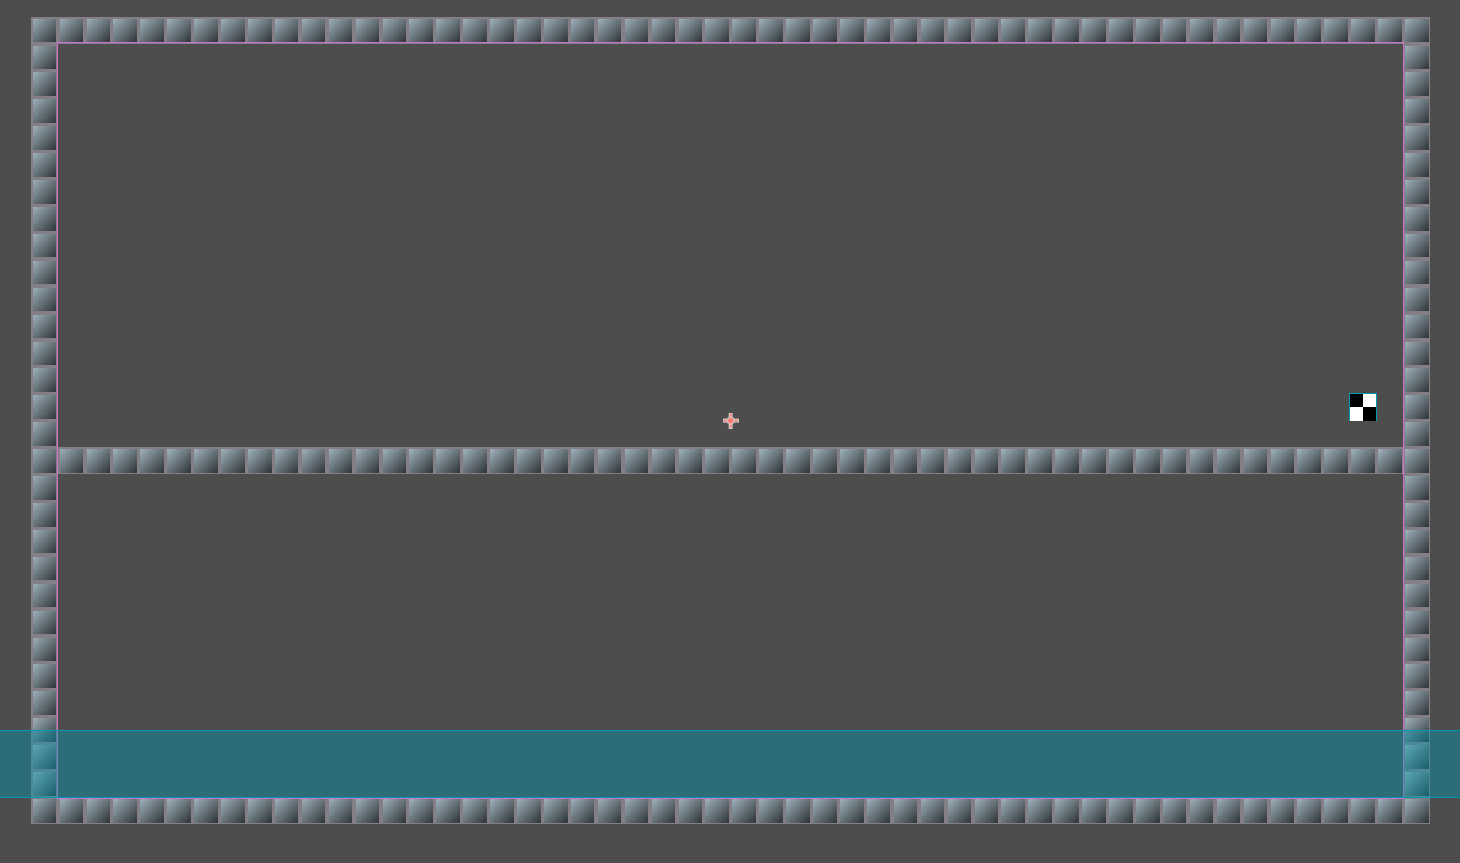
\includegraphics[width=0.8\textwidth]{figures/godot_environment_basic}
    \caption{Basic Godot game environment}
    \label{fig:godot_environment_basic}
\end{figure}

Godot's node based architecture allowed me to neatly lay these all out.

\begin{figure}[h]
    \centering
    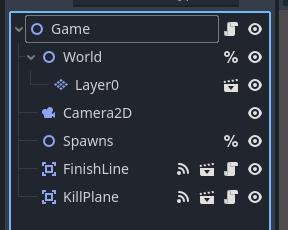
\includegraphics[width=0.8\textwidth]{figures/godot_nodes_basic.png}
    \caption{Godot's node hierarchy for the basic environment}
    \label{fig:godot_nodes_basic}
\end{figure}